\part{System architecture}

\chapter{Microservice architecture}

Microservice architecture is an architectural pattern that arranges an application as a collection of loosely coupled, fine-grained services, communicating through lightweight protocols. One of its goals is to enable teams to develop and deploy their services independently. This is achieved by reducing several dependencies in the codebase, allowing developers to evolve their services with limited restrictions, and hiding additional complexity from users. Consequently, organizations can develop software with rapid growth and scalability, as well as use off-the-shelf services more easily. Communication requirements are reduced. These benefits come with the cost of maintaining decoupling, so a microservice architecture may be suitable only if the application is too complex to manage as a monolith. Interfaces need to be designed carefully and treated as public API. One technique used is having multiple interfaces on the same service or multiple versions of the same service to avoid disrupting existing users of the code.

\begin{figure}
    \centering
    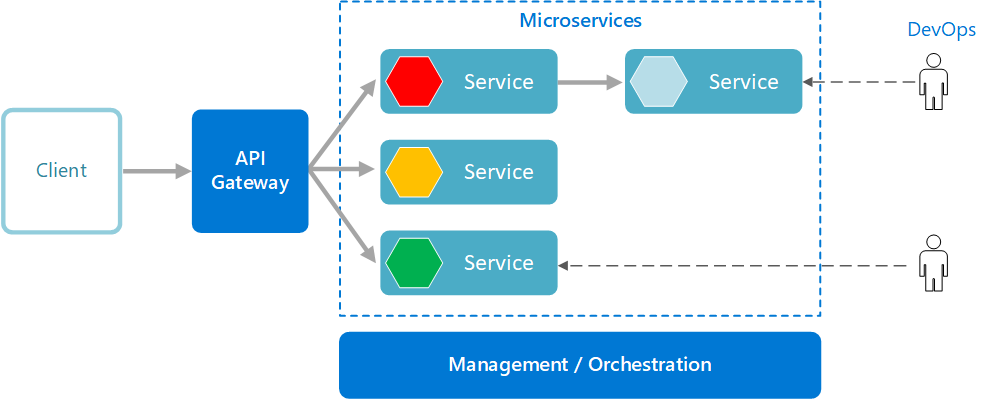
\includegraphics[width=1\linewidth]{images/microservices-architecture.png}
    \caption{Microservices architecture}
    \label{microservices-architecture}
\end{figure}

\textbf{Characteristics of Microservices}
\begin{enumerate}
    \item Componentization via Services: Component is a unit of software that is independently replaceable and upgradeable.

    \item Organized around Business Capabilities: The microservice approach to division is splitting up into services organized by business capability.
    
    \item Products not Projects: This is Amazon’s notion of “you build, you run it” where a development team takes full responsibility for the software in production.
    
    \item Smart endpoints and dumb pipes: Microservices aim to be as decoupled and as cohesive as possible, so they own their own domain logic and receiving a request, applying logic and producing a response with using Restful APIs.
    
    \item Decentralized Governance: Netflix is a good example of an organization that follows this philosophy. Sharing useful and all tested code as libraries, encourages other developers to solve similar problems in similar ways.

    \item Decentralized Data Management: Microservices also decentralize data storage decisions. We can say this approach as a Polyglot Persistence or Polyglot Databases. That means Microservices prefer letting each service manage its own database, either different instances of the same database technology, or entirely different database systems.

    \item Infrastructure Automation: That means automate deployment to each new environment and for every microservices with separately.

    \item Design for failure, Resilience: Microservices design by dealing failures and try to manage failures with managing errors with proper actions. Microservices are also designed to be resilient, meaning that they can continue to operate even if one or more services fail. Because each service operates independently, a failure in one service should not affect the entire application.

    \item Scalable: Each service operates independently, it is possible to scale individual services up or down as needed, without affecting the rest of the application. This allows teams to allocate resources more efficiently and ensure that the application can handle increased traffic or usage.

    \item Technology Agnostic: Different services can be written in different programming languages or use different technology stacks. This makes it easier to choose the right tool for the job, rather than being tied to a particular technology stack.
\end{enumerate}

So these characteristic brings some key benefits;
\begin{itemize}
    \item Code can be updated more easily — new features or functionality can be added without touching the entire application
    \item Teams can use different tech stacks and different programming languages for different components.
    \item Services can be scaled independently, it is reducing the waste and cost associated scale to entire applications because of a single feature might be facing too much load.
    \item Each microservice is highly maintainable and testable — enables rapid and frequent development and deployment
    \item Loosely coupled with other services — enables a team to work independently the majority of time on their service(s) without being impacted by changing to other services and without affecting other services
    \item Independently deployable — enables a team to deploy their service without having to coordinate with other teams
\end{itemize}
So, microservices are an architectural style that emphasizes the decentralization, autonomy, scalability, resiliency, composability, technology agnosticism, and API-first nature of software services. By leveraging these characteristics, teams can build more agile, scalable, and reliable software applications that can be updated and maintained more easily.